
\begin{frame}
	\frametitle{Steepest Descent}
	Most basic iterative technique for solving $\min_\bfx \phi(\bfx)$
	\begin{center}
		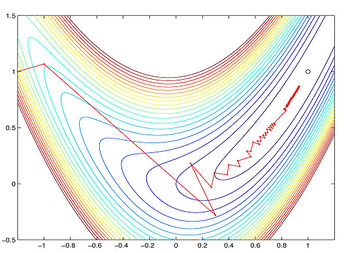
\includegraphics[width=6cm]{steepestDescent.jpg}
	\end{center}
	\begin{equation*}
		\bfx_{j+1} = \bfx_j + \alpha_j \bfd_j \quad \text{ with } \quad \bfd_j =  - \nabla \phi(\bfx_j).
	\end{equation*}
	\pause
	Interpretation 1: $\bfd_{j+1}$ maximizes local descent, i.e., solves
	\begin{equation*}
		\min_{s} \phi(\bfx_j) + \bfd^\top \nabla \phi(\bfx_j) \quad \text{ subject to }\quad \|\bfd\|_2 = 1.
	\end{equation*}
	
	\pause
	
	Interpretation 2: $\bfd_j$ is orthogonal to level sets of $\phi$ at $\bfx_j$.
	
	
\end{frame}